\documentclass[10pt]{article}
\usepackage{graphicx}
\usepackage{amssymb}
\usepackage[fleqn]{amsmath}
\usepackage{nccmath}
\usepackage{cases}
\usepackage{hyperref}
\usepackage{multicol}
\usepackage{tikz}
\usepackage{pgfplots}
\usepackage{enumitem}
\usepackage{pdfpages}
\pgfplotsset{compat=1.18}
\usepackage{float}


\title{\bf Math 151b: Problem Set 5}
\date{2/16/2024}
\author{\bf Owen Jones}
\begin{document}
\maketitle
\textbf{Problem 1}
\begin{enumerate}[label=(\alph*)]
    \item \begin{align*}
        & y_{n+1}-y_n=h[\theta\lambda y_{n+1}+(1-\theta)\lambda y_n]\\
        & y_{n+1}-h\lambda\theta y_{n+1}=y_n+h\lambda(1-\theta) y_n\\
        & y_{n+1}(1-z\theta)=(1+z(1-\theta))y_n\\
        & y_{n+1}=\frac{1+(1-\theta)z}{1-z\theta}y_n
    \end{align*}
    \item \begin{align*}
        & {\lvert w\rvert}^2=w\overline{w}=\frac{1+(1-\theta)z}{1-z\theta}\frac{1+(1-\theta)\overline{z}}{1-\overline{z}\theta}\\
        & =\frac{1+(1-\theta)(z+\overline{z})+{(1-\theta)}^2{\lvert z\rvert}^2}{1-\theta(z+\overline{z})+\theta^2{\lvert z\rvert}^2}\\
        & \Rightarrow {\lvert w\rvert}^2-1=\frac{1+(1-\theta)(z+\overline{z})+{(1-\theta)}^2{\lvert z\rvert}^2}{1-\theta(z+\overline{z})+\theta^2{\lvert z\rvert}^2}-\frac{1-\theta(z+\overline{z})+\theta^2{\lvert z\rvert}^2}{1-\theta(z+\overline{z})+\theta^2{\lvert z\rvert}^2}\\
        & =\frac{(1-2\theta){\lvert z\rvert}^2+(z+\overline{z})}{1-\theta(z+\overline{z})+\theta^2{\lvert z\rvert}^2}=\frac{(1-2\theta){\lvert z\rvert}^2+(z+\overline{z})}{{\lvert 1-\theta z\rvert}^2}\\
        & \text{Because }\theta,1\in\mathbb{R}\Rightarrow \overline{1-\theta z}=1-\theta\overline{z}\\
        & \Rightarrow 1-\theta(z+\overline{z})+\theta^2{\lvert z\rvert}^2=\overline{1-\theta z}(1-\theta z)={\lvert 1-\theta z\rvert}^2\\
    \end{align*}
    If $\lvert w\rvert<1$ then ${\lvert w\rvert}^2-1<0\Leftrightarrow \frac{(1-2\theta){\lvert z\rvert}^2+(z+\overline{z})}{{\lvert 1-\theta z\rvert}^2}<0\\
    \Leftrightarrow (1-2\theta){\lvert z\rvert}^2+(z+\overline{z})<0$.
    \item $(1-2\theta){\lvert z\rvert}^2+(z+\overline{z})=(1-2\theta)z\overline{z}+(z+\overline{z})\\
    =(1-2\theta)z\overline{z}+(z+\overline{z})+\frac{1}{1-2\theta}-\frac{1}{1-2\theta}=(1-2\theta)(z+\frac{1}{1-2\theta})(\overline{z}+\frac{1}{1-2\theta})-\frac{1}{1-2\theta}\\
    =(1-2\theta){\lvert z+\frac{1}{1-2\theta}\rvert}^2-\frac{1}{1-2\theta}$
    \pagebreak
    \item \begin{enumerate}[label=(\roman*)]
        \item Combining (b) and (c) we get\\
        $\lvert w\rvert<1\Leftrightarrow (1-2\theta){\lvert z+\frac{1}{1-2\theta}\rvert}^2-\frac{1}{1-2\theta}<0$\\
        Because $1-2\theta<0\Rightarrow {\lvert z+\frac{1}{1-2\theta}\rvert}^2>{\frac{1}{1-2\theta}}^2$\\
        Taking the square root of both sides $\lvert z-\frac{1}{2\theta-1}\rvert>\frac{1}{2\theta-1}$
        \item Because $1-2\theta>0\Rightarrow {\lvert z+\frac{1}{1-2\theta}\rvert}^2<{\frac{1}{1-2\theta}}^2$\\
        Taking the square root of both sides $\lvert z+\frac{1}{1-2\theta}\rvert<\frac{1}{1-2\theta}$
        \item For $\theta=\frac{1}{2}$ we need $\Re(z)<0$ from the trapezoidal stability region lecture note.
    \end{enumerate}
\end{enumerate}
\textbf{Problem 2}
\begin{enumerate}[label=(\alph*)]
    \item Boundary Region
    \begin{figure}[H]
        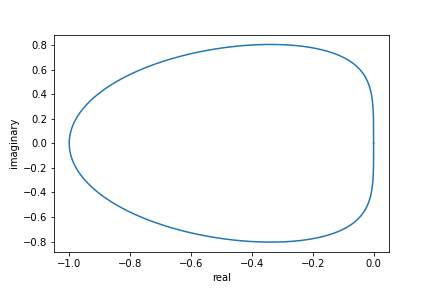
\includegraphics[scale=0.5]{AB_2_boundary.png}
    \end{figure}
    $y_{n+2}-y_{n+1}=h(\frac{3}{2}\lambda y_{n+1}-\frac{1}{2}\lambda y_n)\\
    \Rightarrow y_{n+2}-(1+\frac{3}{2}z)y_{n+1}+\frac{1}{2}z y_n=0\\
    \Rightarrow \rho(r;z)=r^2-(1+\frac{3}{2}z)r+\frac{1}{2}z\\
    \text{Boundary }z=\frac{e^{2\theta i}-e^{\theta i}}{\frac{3}{2}e^{\theta i}-\frac{1}{2}}\text{ for }\theta\in[0,2\pi]\\
    r=\frac{1+\frac{3}{2}z+\sqrt{\frac{9}{4}z^2+z+1}}{2},\frac{1+\frac{3}{2}z-\sqrt{\frac{9}{4}z^2+z+1}}{2}$\\
    stability region inside boundary because $z=-0.5+0i$ satisfies root condition.\\
    %Stability Region:\\
    %$R=\{z\in\mathbb{C}:\lvert\frac{1+\frac{3}{2}z+\sqrt{\frac{9}{4}z^2+z+1}}{2}\rvert<1,\lvert\frac{1+\frac{3}{2}z-\sqrt{\frac{9}{4}z^2+z+1}}{2}\rvert<1\}$\\
    \pagebreak
    \item Boundary Region
    \begin{figure}[H]
        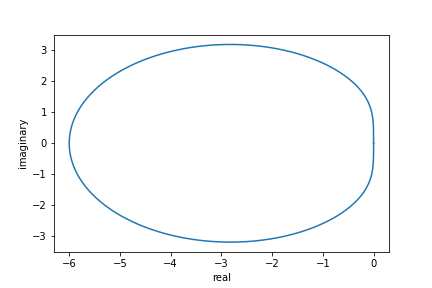
\includegraphics[scale=0.5]{AM_2_boundary.png}
    \end{figure}
    $y_{n+2}-y_{n+1}=h(\frac{5}{12}\lambda y_{n+2}+\frac{8}{12}\lambda y_{n+1}-\frac{1}{12}\lambda y_n)\\
    \Rightarrow (1-\frac{5}{12}z)y_{n+2}-(1+\frac{8}{12}z)y_{n+1}+\frac{1}{12}z y_n=0\\
    \Rightarrow \rho(r;z)=(1-\frac{5}{12}z)r^2-(1+\frac{8}{12}z)r+\frac{1}{12}z\\
    r=\frac{1+\frac{2}{3}z+\sqrt{\frac{23}{48}z^2+z+1}}{2-\frac{5}{6}z},\frac{1+\frac{2}{3}z-\sqrt{\frac{23}{48}z^2+z+1}}{2-\frac{5}{6}z}$\\
    stability region inside boundary because $z=-3+0i$ satisfies root condition.\\
    %Stability Region:\\
    %$R=\{z\in\mathbb{C}:\lvert\frac{1+\frac{2}{3}z+\sqrt{\frac{23}{48}z^2+z+1}}{2-\frac{5}{6}z}\rvert<1,\lvert\frac{1+\frac{2}{3}z-\sqrt{\frac{23}{48}z^2+z+1}}{2-\frac{5}{6}z}\rvert<1\}$\\
\end{enumerate}
\textbf{Problem 3}
\begin{enumerate}[label=(\alph*)]
    \item \begin{align*}
        & y_{n+1}=y_n+hk_2\\
        &=y_n+h\lambda(y_n+hk_1/2)\\
        &=y_n+h\lambda(y_n+h\lambda y_n/2)\\
        &=y_n+z(y_n+z y_n/2)\\
        &=(1+z+\frac{z^2}{2})y_n
    \end{align*}
    \item \begin{align*}
        &y_{n+1}=y_n+h(\frac{1}{6}k_1+\frac{4}{6}k_2+\frac{1}{6}k_3)\\
        &=y_n+h(\frac{1}{6}\lambda y_n+\frac{4}{6}\lambda(y_n+h\lambda y_n/2)+\frac{1}{6}\lambda(y_n-h\lambda y_n+2h\lambda(y_n+h\lambda y_n/2)))\\
        &=y_n+(\frac{1}{6}z y_n+\frac{4}{6}z(y_n+z y_n/2)+\frac{1}{6}z(y_n-z y_n+2z(y_n+z y_n/2)))\\
        &=(1+\frac{1}{6}z +\frac{4}{6}z(1+z/2)+\frac{1}{6}z(1-z+2z(1+z/2)))y_n\\
        &=(1+\frac{1}{6}z +\frac{4}{6}(z+z^2/2)+\frac{1}{6}(z+z^2+z^3))y_n\\
        &=(1+z+\frac{z^2}{2}+\frac{z^3}{6})y_n\\
    \end{align*}
    \item \begin{align*}
        &y_{n+1}=y_n+h(\frac{1}{6}k_1+\frac{2}{6}k_2+\frac{2}{6}k_3+\frac{1}{6}k_4)\\
        &h\frac{1}{6}k_1=\frac{z}{6}y_n\\
        &h\frac{2}{6}k_2=(\frac{2z}{6}+\frac{z^2}{6})y_n\\
        &h\frac{2}{6}k_3=(\frac{2z}{6}+\frac{z^2}{6}+\frac{z^3}{12})y_n\\
        &h\frac{1}{6}k_4=(\frac{z}{6}+\frac{z^2}{6}+\frac{z^3}{12}+\frac{z^4}{24})y_n\\
        &\Rightarrow y_{n+1}=y_n+\frac{z}{6}y_n+(\frac{2z}{6}+\frac{z^2}{6})y_n+(\frac{2z}{6}+\frac{z^2}{6}+\frac{z^3}{12})y_n+(\frac{z}{6}+\frac{z^2}{6}+\frac{z^3}{12}+\frac{z^4}{24})y_n\\
        &=(1+z+\frac{z^2}{2}+\frac{z^3}{6}+\frac{z^4}{24})y_n
    \end{align*}
    \pagebreak
    \item The area of the stability regions increases when we use higher degree polynomials.
    \begin{figure}[H]
        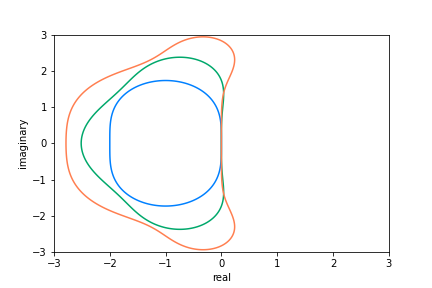
\includegraphics[scale=0.5]{RK_boundaries.png}
    \end{figure}
\end{enumerate}
\textbf{Problem 4}
\begin{enumerate}[label=(\alph*)]
    \item If $y(t)={(0,0,1)}^\top$ then\\
    $y'(t)={(-\alpha\cdot 0+\beta \cdot 0\cdot 1,\alpha\cdot 0-\beta \cdot 0\cdot 1-\gamma\cdot 0^2,\gamma\cdot 0^2)}^\top ={(0,0,0)}^\top$\\
    $\displaystyle\frac{d}{dt}[\sum_{i=1}^{3}y(t)]=\sum_{i=1}^{3}y'(t)=(-\alpha y_1+\beta y_2y_3)+(\alpha y_1-\beta y_2y_3-\gamma y_2^2)+(\gamma y_2^2)=0$\\
    Thus, by the FTC $\displaystyle \sum_{i=1}^{3}y(t)-\sum_{i=1}^{3}y(0)=\int_{0}^{t}\sum_{i=1}^{3}y'(t)dt=0\Rightarrow \sum_{i=1}^{3}y(t)=\sum_{i=1}^{3}y(0)=1$ for all $t>0$.\\
    Since $\displaystyle \sum_{i=1}^{3}\mathbf{y}_e=1$ the reaction model admits the unique steady state $\mathbf{y}_e={(0,0,1)}^\top$.\\
    \item Solver uses $30001$ time steps. The numerical solution doesn't appear to be anywhere close to the steady state solution. Used a max step size of $10^{-4}$
    \item Solver uses $27$ time steps. Requires significantly fewer time steps used then for part (b). Also, doesn't appear to be closer to the steady state.
    \pagebreak
    \item I used a final time of $T=3\times 10^4$ to obtain a $y_3(T)\approx 0.95$. The solver only used $95$ time steps. 
    \begin{figure}[H]
        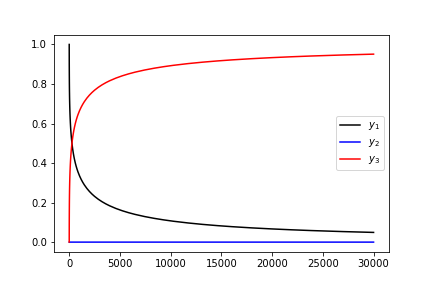
\includegraphics[scale=0.5]{stiff_solver_chemical_reaction_rate.png}
    \end{figure}
\end{enumerate}
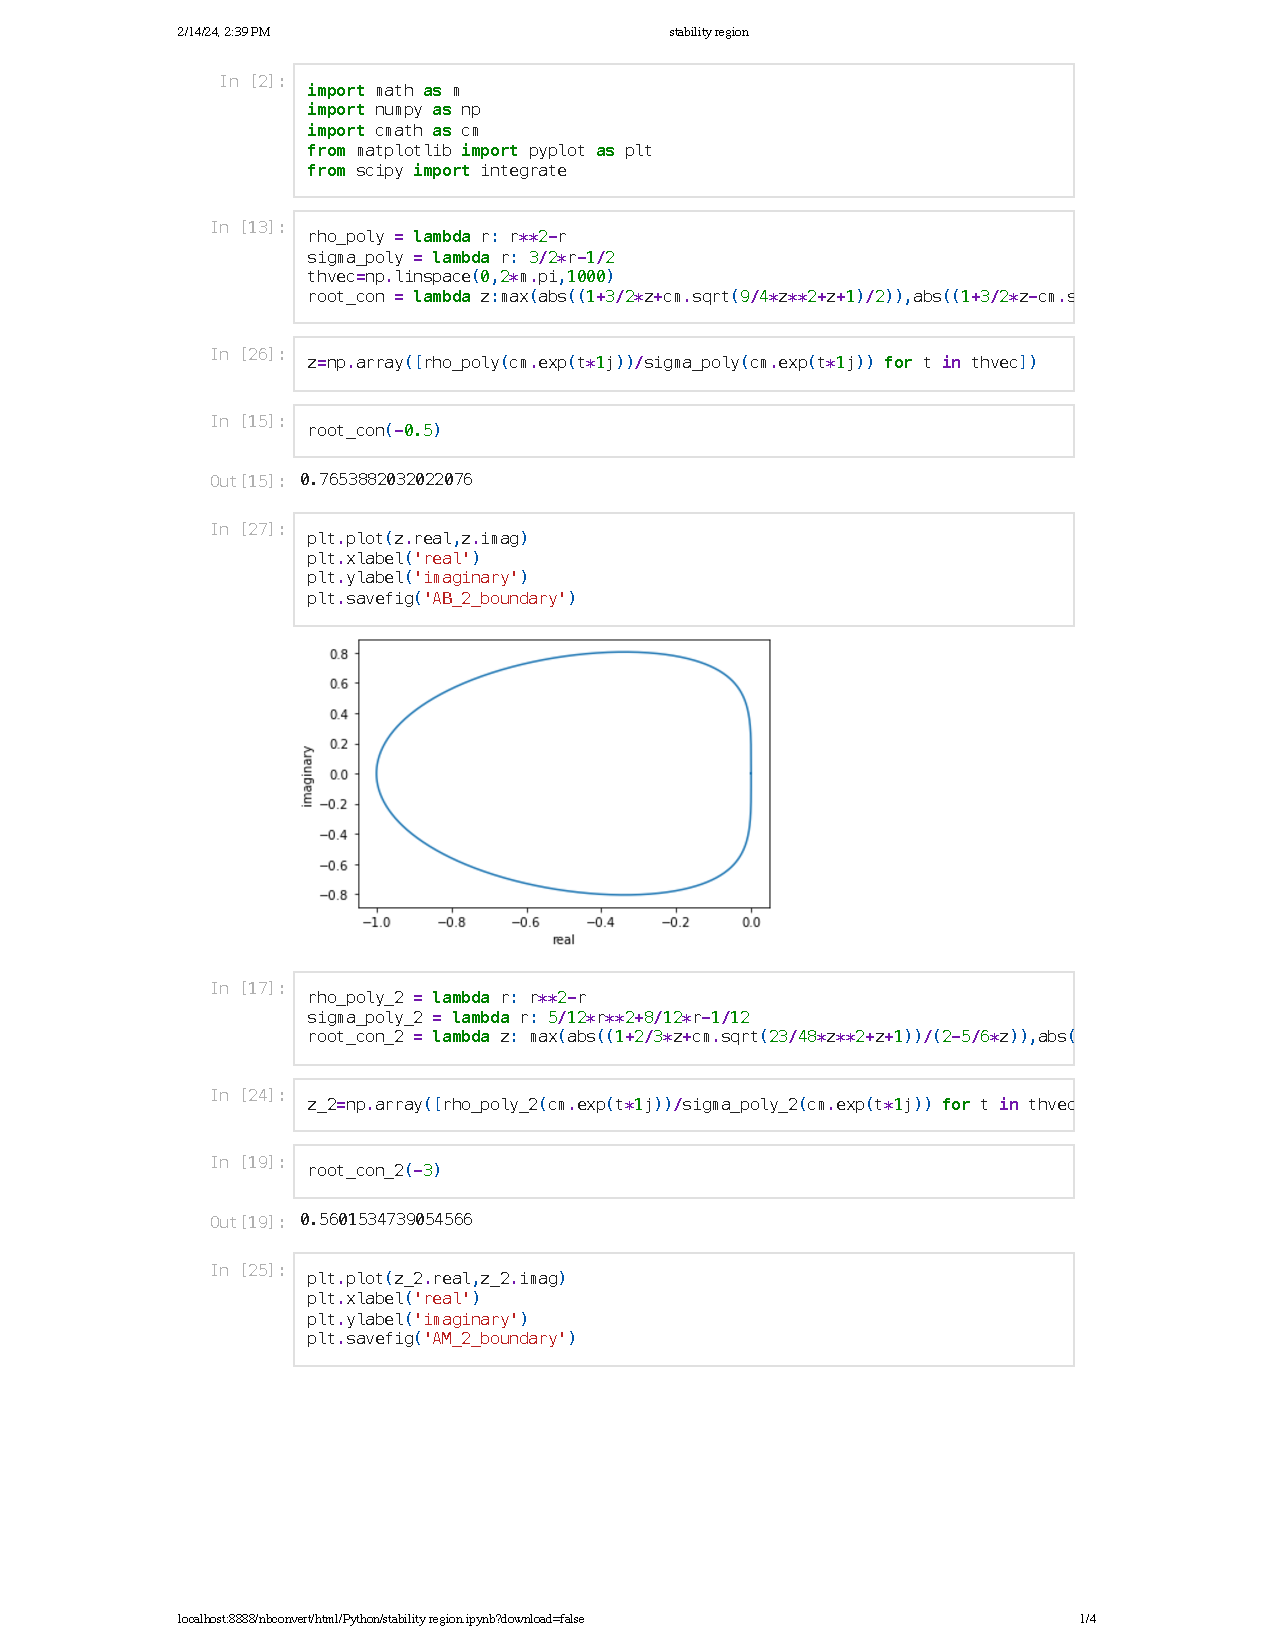
\includepdf[pages=-]{stability region.pdf}
\end{document}